%%%%%%%%%%%%%%%%%%%%%%%%%%%%%%%%%%%%%%%%%%%%%%%%%%%%%%%%%%%%%%%%%%%%%%%%%%%%%%%%
%2345678901234567890123456789012345678901234567890123456789012345678901234567890
%        1         2         3         4         5         6         7         8

\documentclass[letterpaper, 10 pt, conference]{ieeeconf} 
\usepackage{times}
\usepackage{algorithmic}
\usepackage{algorithm}
\usepackage{subcaption}
%\documentclass[a4paper, 10pt, conference]{ieeeconf}      % Use this line for a4 paper

% See the \addtolength command later in the file to balance the column lengths
% on the last page of the document

% The following packages can be found on http:\\www.ctan.org
%\usepackage{graphics} % for pdf, bitmapped graphics files
%\usepackage{epsfig} % for postscript graphics files
%\usepackage{mathptmx} % assumes new font selection scheme installed
%\usepackage{times} % assumes new font selection scheme installed
%\usepackage{amsmath} % assumes amsmath package installed
%\usepackage{amssymb}  % assumes amsmath package installed
\usepackage{mathtools}
\usepackage{amsmath}
\usepackage{amsfonts}
\usepackage{color}
\usepackage{amssymb}
\DeclareMathOperator*{\argmin}{\arg\!\min} 
\DeclareMathOperator*{\argmax}{\arg\!\max} 

% \title{\LARGE \bf
% Rapidly Exploring Learning Trees
% }
\IEEEoverridecommandlockouts                              % This command is only needed if 
                                                          % you want to use the \thanks command

\overrideIEEEmargins  

\title{\LARGE \bf
Rapidly Exploring Learning Trees
}


\author{Kyriacos Shiarlis$^{1}$ Joao Messias$^{1}$ Shimon Whiteson$^{2}$% <-this % stops a space
% \thanks{*This work was not supported by any organization}% <-this % stops a space
\thanks{$^{1}$Informatics Institute, University of Amsterdam, The Netherlands,
         {\tt\small \{k.c.shiarlis,j.messias\}@uva.nl}}%
\thanks{$^{2}$Department of Computer Science, University of Oxford, United Kingdom,
         {\tt\small shimon.whiteson@cs.ox.ac.uk}}%
}



% \author{Kyriacos Shiarlis \\
% University of Amsterdam \\
% k.c.shiarlis@uva.nl
% \And 
% Joao Messias \\
% University of Amsterdam \\ 
% jmessias@uva.nl 
% \And
% Shimon Whiteson \\
% University of Oxford \\
% shimon.whiteson@cs.ox.ac.uk 
% }
\newcommand{\jm}[1]{\textcolor{blue}{Joao: #1}}

\newcommand{\sw}[1]{\textcolor{red}{SW: #1}}
\newcommand{\ks}[1]{\textcolor{green}{KS: #1}}


\begin{document}

\maketitle

\thispagestyle{empty}
\pagestyle{empty}


%%%%%%%%%%%%%%%%%%%%%%%%%%%%%%%%%%%%%%%%%%%%%%%%%%%%%%%%%%%%%%%%%%%%%%%%%%%%%%%%
\begin{abstract}
Inverse Reinforcement Learning (IRL) for path planning enables robots to learn cost functions for difficult tasks from demonstration, instead of hard-coding them. However, IRL methods face practical limitations that stem from the need to repeat costly planning procedures.
In this paper, we propose Rapidly Exploring Learning Trees (RLT$^*$), which learns the cost functions of Rapidly Exploring Random Trees (RRT) from demonstration, thereby making inverse learning methods applicable to more complex tasks. Our approach extends Maximum Margin Planning to work with RRT$^*$ cost functions. Furthermore, we propose a caching scheme that greatly reduces the computational cost of this approach. Experimental results on simulated and real-robot data from a social navigation scenario show that RLT$^*$ achieves better performance at lower computational cost than existing methods.  We also successfully deploy control policies learned with RLT$^*$ on a real telepresence robot.


\end{abstract}


%%%%%%%%%%%%%%%%%%%%%%%%%%%%%%%%%%%%%%%%%%%%%%%%%%%%%%%%%%%%%%%%%%%%%%%%%%%%%%%%
\section{Introduction}

Learning from demonstration (LfD) \cite{argall2009survey} is of great interest to roboticists because it can avoid the need for tedious manual programming of complex behaviours. While most LfD methods rely on supervised learning (i.e., behavioural cloning) to directly learn policies, certain approaches, namely inverse optimal control (IOC) \cite{kalman1964linear} and inverse reinforcement learning (IRL) \cite{abbeel2004apprenticeship} instead learn \emph{cost functions} from demonstration, which are then used to \emph{plan} the robot's behaviour. 

In addition, learned cost functions are often useful even when the environment changes.  For example, if the friction in a robot's wheels changes due to wear and tear, the optimal policy will change but the cost function will not. Thus, a robot trained via supervised learning would need to learn a new policy, while a robot trained via IRL could simply replan on the new dynamics with its existing cost function. In addition, cost functions are thought to be more succinct representations of the aims of the agent \cite{abbeel2004apprenticeship}. For example, a robot whose aim is to reach a goal as fast as possible may have a simple cost function but a complex policy. 

IRL is an iterative process that, in an inner loop, solves the forward planning problem (i.e., finds an optimal policy under the current cost function) and subsequently, in an outer loop, updates the current cost function. This process repeats until convergence. For continuous domains such as robotics, solving the planning problem exactly is typically intractable. The domain can be discretised but doing so scales poorly in the dimensionality, necessitating a coarse discretisation that yields poor performance.  Consequently, in robotics, planning is often done using sample-based, single-query motion planners, such as Rapidly Exploring Random Trees (RRTs) \cite{lavalle1998rapidly} and their variants \cite{karaman2011sampling}. Such methods can cope with high-dimensional continuous domains and elegantly handle obstacles in the environment and motion constraints on the robot.

%  IRL for example requires modeling the task as a Markov decision process (MDP), which is typically impractical in robotics, for several reasons.  Firstly, an MDP assumes full observability. Secondly, planning in an MDP, which IRL methods must do repeatedly, is costly, especially in continuous and high-dimensional domains. Finally, the lack of scalability and the assumption of full observability prohibit the accurate modeling of all aspect of the environment that a robot is expected to operate in. 

% For these reasons, several researchers have proposed replacing the planning step in IRL with more convienient planners, e.g., Maximum Margin Planning (MMP)~\cite{ratliff2006maximum} uses A$^*$ search for planning. This avoids the need to do all the planning in advance, as is typical when solving an MDP. It also avoids the need to model all aspects of the environment since the robot can quickly replan its trajectory to account for uncertainty. However, deterministic search methods such as A$^*$ require discretisation of the state space, and quickly run into scalability problems as the discretisation becomes finer. 

In this paper, we propose a new approach to IRL that enables the use of RRT$^*$ \cite{karaman2011sampling}, the optimality-driven variant of RRT, in the planning step.  First, we propose Approximate Maximum Margin Planning (AMMP), a variant of Maximum Margin Planning (MMP) \cite{ratliff2006maximum} that does not require optimal planning.  Second, we propose a caching scheme that both improves performance and reduces computational cost when RRT$^*$ is used within AMMP. The resulting algorithm, which we call Rapidly Exploring Learning Trees (RLT$^*$),  allows computationally efficient IRL in high-dimensional, continuous domains with obstacles and motion constraints. 

We evaluate RLT$^*$ on real and simulated data from a social navigation scenario. The results demonstrate that, in the absence of obstacles and motion constraints, RLT$^*$ performs better and is faster than both MMP and RLT$^*$ without caching. Furthermore, we show that RLT$^*$, unlike MMP, can learn cost functions in robotic tasks with obstacles and motion constraints. Finally, we deploy our method on a real telepresence robot using data from human demonstrations.

% In path planning, Rapidly Exploring Random Trees (RRTs)~\cite{lavalle1998rapidly} are popular because they cope well with continuous and high-dimensional domains. The RRT$^*$ algorithm , which extends RRTs to incorporate a cost function, is especially effective. However, the cost functions used by RRT$^*$ are typically simple and hand-coded and, to our knowledge, no methods have been developed to learn RRT$^*$ cost functions from demonstrations.


% In this paper, we propose Rapidly Exploring Learning Trees (), which learns RRT$^*$ cost functions from demonstration. Specifically we modify Maximum Margin Planning to use RRT$^*$ as a planner.  RLT$^*$ requires no additional planner assumptions other than those inherent in RRT$^*$, making it particularly easy to implement. 

\section{Related Work \label{sec:related_work}}


Substantial research has applied IRL to robotics \cite{henry2010learning,abbeel2008apprenticeship,vasquez2014inverse}.
A big challenge in doing so is solving the forward planning problem under the current cost function at every iteration. The planning problem is especially intractable in robotics where the state-action spaces encountered are continuous and high dimensional. %Researchers thus resort to assumptions and approximations which reduce the computational cost of the procedure while allowing for high quality solutions. 

One approach is to discretise the state-action spaces and solve the resulting Markov decision process (MDP). However, in high-dimensional tasks, fine discretisations render planning intractable and coarse discretisations yield poor performance.

Some methods that use discretisation formulate the problem such that only an open-loop path (rather than a closed-loop policy) is required. Then, given deterministic dynamics, planning can be performed using A$^*$ \cite{ratliff2006maximum}, allowing realistic problems to be tackled. We take a similar approach but, by planning using RRT$^*$, we expand on the possibilities of the tasks that can be learned. \sw{This is confusing: paths are easier to plan so can scale better wrt dimensionality?  But still require discretisation and so not as scalable as RRT?  Needs to be made much clearer.}

Another approach is to use hybrid planners. Inverse Optimal Heuristic Control \cite{ratliff2009inverse} models the long-term goals of the agent as a coarsely discretised MDP, to ensure tractability, while using supervised learning to determine the local policy of the agent at each state. Graph-Based IOC \cite{byravan2015graph} uses discrete optimal control on a coarse graph and the actual path is executed using local trajectory optimisation techniques such as CHOMP \cite{ratliff2009chomp}, which would otherwise suffer from local minima. However, these methods employ complex and domain-specific planning formulations that are not suitable for all robotics tasks. By contrast, our approach employs widely used planners, making it versatile and easy to implement. 

Another recent method is that Adaptive State Graphs \cite{okallearning}, which builds a state-action controller graph before doing any learning. This controller graph is akin to \emph{options} in semi-Markov decision processes, and allows for a more flexible representation of the state-action space. However, the controller used to learn underlying cost function is different from the one used to execute the robot's behaviour. This can have adverse effects since IRL  assumes that the demonstration paths came from the same planner used during learning.  Instead of building a controller graph first and then using a different controller to optimise trajectories, RLT$^*$ builds a controller tree on the fly and uses the same planner for learning and execution.

 All of the above methods require require a model of the dynamics of the system. By contrast, model-free IRL uses importance sampling to deal with high-dimensional state-action spaces with unknown dynamics \cite{boularias2011relative,kalakrishnan2013learning}. Instead of performing a full planning procedure at each iteration, model free IRL samples trajectories, usually starting from the initial conditions observed in the data. The probability of these trajectories is weighted according to the current cost function, which is then updated to make trajectories closer to the data more likely. A big challenge is to find an appropriate importance distribution at each iteration. \cite{finn2016guided} considers guiding the importance distribution by simultaneously learning a good policy under the current cost function and using it as an adaptive importance sampler. However the method uses a modified version of Linear Quadratic Regulator control to derive policies, which means that these policies are only locally optimal. This means that they can produce highly suboptimal paths in or even fail in the presence of obstacles in the environment. By contrast, if obstacles are are static and mapped RRTs, have a natural way of dealing with them, while also being asymptotically optimal.






% Because of the need to model the environment as an MDP, researchers usually discretise the state-action space. This introduces several key limitations. First, the size of the state-action space encountered in robotics is often prohibitive for such models. Second, the specific not all physical aspects of the robot can be easily expressed by such representations, introducing non-Markovian dynamics. 

% \ks{Depending on the state-action space discretisation, past actions can infuence how easy it is to move to any a subsequent state. However the transition function only considers only one action in the past, and it is therefore an expectation over possible past configurations. As a result it tends to give the wrong probability distribution over next states for the actual physical system. Do I have to explain this in detail? Maybe Joao has a citation from his research?}

% To apply IRL to more realistic situations, researchers usually try to replace the MDP model while retaining the main idea behind IRL, i.e., learning the underlying cost function of a planner using data from demonstrations. Maximum Entropy IRL \cite{ziebart2010modelingthesis} works in domains with linear continuous dynamics with the optimal controller being a Linear-Quadratic Regulator. Since linear dynamics are hard to come by in robotics, \cite{2012-cioc} considers locally linear approximations. These bring about locally consistent rewards and achieve good performance in a range of tasks that were previously too hard for MDPs. However, the optimisation of the cost function using such planners is not guaranteed to be optimal. As our method is based on an RRT$^*$ planner, it is asymptotically optimal.

% Other approaches to the problem use hybrid planners. Inverse Optimal Heuristic Control \cite{ratliff2009inverse} models the long-term goals of the agent as a coarse state MDP, to ensure tractability, while using supervised learning to determine the local policy of the agent at each state. Graph-Based IOC \cite{byravan2015graph} uses discrete optimal control on a coarse graph and the actual path is executed using local trajectory optimisation techniques such as CHOMP \cite{ratliff2009chomp}, which would otherwise suffer from local minima. The method is effective in robotic manipulation tasks with many degrees of freedom.  However, these methods employ complex and domain-specific planning formulations that are not suitable for all robotics tasks. The method presented here employs widely used planners, making it versatile and easy to implement. 

% Another more recent graph-based concept is that of Adaptive State Graphs \cite{okallearning}, which build a controller graph before doing any learning. This controller graph is akin to \emph{options} in semi-Markov decision processes, and allows for a more flexible representation of the state-action space. However, the controller used to learn underlying cost function is not the same as the one used to execute the robot's behaviour. This can have adverse effects since an implicit assumption of IRL is that the demonstration paths came from the same planner that we use during learning. This planner has specific representations, such as discretisation and parameters such as the discount factor. If these change, different policies arise. As a result a path that was optimal under a certain planner ceases to be optimal under another.



\section{Background}
We begin with background on path planning and inverse reinforcement learning for path planning.

\subsection{Path Planning \label{subsec:path_planning}}
Path planning occurs in a space $\mathcal{S}$ of possible robot configurations. A configuration $s \in \mathcal{S}$ is usually continuous, and often represents spatial quantities such as position and orientation. A path planner seeks an obstacle-free path $\zeta_{o,g} = (s_1,s_2,s_3$ $\ldots,s_{l_{\zeta}}) $ of length $l_{\zeta}$, from an initial configuration $o = s_1$ to a goal configuration  $g =s_{l_{\zeta}}$. When the initial and goal configurations are implied, we refer to a path as $\zeta$.

As there could be several paths to the goal, planners often employ a \emph{cost functional}, $C(\zeta)$, which typically sums the costs between two subsequent configurations $c(s_i,s_j)$:
\begin{equation}
	C(\zeta) = \sum_{i=1}^{l_{\zeta}-1} c(s_i,s_{i+1}).
\end{equation}
This cost functional is similar to the one used in optimal control and analogous to the return used in reinforcement learning. Given the cost functional, the path planner seeks an optimal path $\zeta^*$, which satisfies,
\begin{equation}
 	\zeta^*_{o,g} = \argmin_{\zeta_{o,g} \in Z_{o,g}} C(\zeta). \label{eq:back_plan}
\end{equation}
$Z_{o,g}$ is the set of possible paths such that $s_1 = o, s_{l_\zeta} = g$.

Many path planning algorithms discretise $\mathcal{S}$ and use graph search algorithms like A$^*$ to find the optimal path. Under mild assumptions, these approaches are guaranteed to find the best path on the graph, therefore solving \eqref{eq:back_plan} for a subset $\tilde{Z}_{o,g} \subset Z_{o,g}$, whose size depends on the discretisation. However, such methods scale poorly in the size of $\mathcal{S}$. Furthermore, such algorithms ignore motion constraints as they assume all nodes in the graph can be reached by its neighbours in exactly the same way. \jm{Is this true, though? The A* node expansion phase would take care of this, as long as there is some state-dependent expansion mechanism it should be fine, no?} This assumption does not hold, e.g., for non-holonomic robots, where the ortientation at each node places constraints on how it can be reached. In this new constrained space it is less straightforward to define actions and neighbouring nodes. 

These drawbacks motivate \emph{sample-based} path planning algorithms such as RRT$^*$  \cite{karaman2011sampling}. Instead of building a graph and then searching it, RRT$^*$ builds a tree on the fly and keeps track of the current best path. The algorithm consists of two interleaved steps. 

The first step is \emph{sampling}. A random point $s_{rand}$ is sampled from the configuration space. Next, the closest point $s_{closest}$, already in the existing vertex set $V$ is determined and a new point $s_{new}$ is created by \emph{steering} from  $s_{closest}$ to $s_{rand}$. In a Euclidean space, steering between two points means simply connecting them with a straight line. However, if orientations and motion constraints are used, then becomes more complex. Finally, the sampling step determines the points, $S_{near}$, within a given radius of $s_{new}$.

The second step is \emph{rewiring}, which determines which points in $S_{near}$ we should connect to $s_{new}$, i.e., it determines which path to $s_{new}$ results in a lowest cost path. Finally, we repeat this step for the parents of $S_{near}$. Thus, the tree is rewired locally around the new point, such that lower global cost paths arise.

Alternating between these two steps for a given time budget $T$ solves \eqref{eq:back_plan} for a subset $\tilde{Z}_{o,g}$ that is determined by the randomly sampled points. As $T \rightarrow \infty$, RRT$^*$ minimises over the entire $Z_{o,g}$, i.e., it is asymptotically optimal in time \cite{karaman2011sampling}. By contrast, A$^*$ is asymptotically optimal in resolution.


% and PRM$^*$. The application focus of this paper is social robotic navigation, which typically consists of highly non-static environments. Therefore multi-query roadmap methods such as PRM$^*$ are not appropriate, since we would need to repeat the learning phase of the algorithm every time as the environment changes. As a result this paper employs RRT$^*$ as the underlying planner for the cost function learning process. 


%  RRT$^*$ is also asymptotically optimal, i.e., it is guranteed to find an optimal path in $\mathcal{S}$ as the sampling time goes to infinity. Many variants of RRT$^*$ provide improved performance and faster convergence in practice by, for example, heuristically shriking the sampling space \cite{gammell2014informed}.

% The most significant difference between A$^*$ and RRT$^*$ is that while former is deterministic, the latter is probabilistic. It is important to understand how this distinction affects learning.

% Comparing A$^*$ and RRT$^*$ in terms of optimality  . . In other words, the RRT$^*$ is asymptotically optimal as a function of sampling time and A$^*$ is asymptotically optimal as a function of resolution. %This distinction will become very important when we attempt to learn cost functions for these planners in the next section.

\subsection{IRL for Path Planning \label{subsec:inverse_problem}}
In path planning, we are given a cost function and must find a (near) optimal path to the goal. In the inverse problem, we are given example paths and must find the cost function for which these paths are (near) optimal.  The example paths comprise a dataset $\mathcal{D} = (\zeta^1_{o_1,g_1},\zeta^2_{o_2,g_2}...\zeta^D_{o_D,g_D})$ where $\zeta^i_{o_i,g_i}$ is an example path with initial and final configurations $o_i$ and $g_i$. We assume the unknown cost function is of the form,
\begin{equation}
	c(s_i,s_j) = \mathbf{w}^T \mathbf{f}(s_i,s_j), \label{eq:inner_prod}
\end{equation}
where $\mathbf{f}(s_i,s_j)$ is a $K$-dimensional vector of features that encode different aspects of the configuration pair and $\mathbf{w}$ is a vector of unknown weights to be learned. Since $\mathbf{w}$ is independent of the configuration, we can express the total cost of the path in a parametric form:

\begin{equation}
	C(\zeta) = \mathbf{w}^T\sum_{i=0}^{l_{\zeta}-1} \mathbf{f}(s_i,s_{i+1}) := \mathbf{w}^T \mathbf{F}(\zeta),
\end{equation}
where $\mathbf{F}(\zeta)$ is the \emph{feature sum} of the path.

While many formulations of the inverse problem exist, the general idea is to find a weight vector that assigns less cost to the example paths than all other possible paths with the same initial and goal configuration.  This can be formalised by a set of inequality constraints:

\begin{equation}
	C(\zeta^i_{o_i,g_i}) \leq  C(\zeta) \quad \forall \zeta \in Z_{o_i,g_i}  \quad \forall i. \label{eq:const1}
\end{equation}
The constraint is an inequality because $Z_{o_i,g_i}$ contains only paths available to the planner and thus may not include the example path $\zeta^i_{o_i,g_i}$.
$Z_{o_i,g_i}$ can be large but if we have an optimisation procedure that solves \eqref{eq:back_plan}, it is enough to satisfy, 
\begin{equation}
	C(\zeta^i_{o_i,g_i}) \leq \min_{\zeta \in Z_{o_i,g_i}} C(\zeta) \quad \forall i, \label{eq:const}
\end{equation}

Maximum Margin Planning (MMP) \cite{ratliff2006maximum} introduces a margin function $L_i(\zeta)$ that decreases the cost of the proposed path $\zeta$ if it is dissimilar to $\zeta^i_{o_i,g_i}$. For example, $L_i(\zeta)$ could be $-1$ times the number of configurations in the demonstration path not visited by $\zeta$. As in Support Vector Machines, requiring the model to fit the data well even in the presence of a margin improves generalisation. Furthermore, the margin helps address the ill-posed nature of IRL, i.e., many cost functions are consistent with the demonstrated behaviour. Formally, MMP solves the following optimisation problem:
\begin{equation}
	\argmin_{\mathbf{w},\tau} \frac{1}{2}||\mathbf{w}||^2 + \frac{\lambda}{D} \sum_i \tau_i \label{eq:mas_marg}
\end{equation}
\begin{equation}
	\text{s.t.} \quad C(\zeta^i_{o_i,g_i}) - \tau_i \leq \min_{\zeta \in Z_{o_i,g_i}} C(\zeta) + L_i(\zeta) \quad \forall i,
\end{equation}
where $\tau_i$ are slacks that can be used to relax the constraints. Rearranging the inequality in terms of the slacks yields:

\begin{equation}
	 \quad C(\zeta^i_{o_i,g_i}) - \min_{\zeta \in Z_{o_i,g_i}} C(\zeta) + L_i(\zeta)  \leq \tau_i  \quad \forall i.
\end{equation}
Consequently, the $\mathbf{w}$ minimising:
\begin{equation}
	\frac{1}{2}||\mathbf{w}||^2 + \frac{\lambda}{D} \sum_i \big( C(\zeta^i_{o_i,g_i}) - \min_{\zeta \in Z_{o_i,g_i}}\big(C(\zeta) + L_i(\zeta)\big) \big) \big. \label{eq:unconstrained}
\end{equation}
also minimises \eqref{eq:mas_marg}, i.e., the slacks are tight.
The minimum can be found by computing a subgradient and performing gradient descent on the above objective:
\begin{equation}
	\nabla_{\mathbf{w}} =\mathbf{w} +  \frac{\lambda}{D} \sum_{i=0}^D F(\zeta^i_{o_i,g_i}) - F(\tilde{\zeta}^*_{o_i,g_i}), \label{eq:update1}
\end{equation}
where,
\begin{equation}
	\tilde{\zeta}^*_{o_i,g_i} = \argmin_{\zeta \in Z_{o_i,g_i}} C(\zeta) + L_i(\zeta). \label{eq:augmented_max}
\end{equation}

The inverse problem can therefore be seen as an iterative procedure that first solves \eqref{eq:augmented_max} in the inner loop while keeping the weights constant. Given that solution, it then updates the weights using \eqref{eq:update1} in the outer loop. The weights at convergence represent the cost function that is used to plan future behaviour. In \cite{ratliff2006maximum}, A$^*$ search was used for planning in the inner loop, assuming that the domain contained acyclic positive costs. In this paper, we make the same assumptions but develop methods that use RRT$^*$ for planning.

\section{Method}
	In this section, we propose Rapidly Exploring Learning Trees (RLT$^*$).  We first propose a generic extension to MMP that we call Approximate Maximum Margin Planning.  We then show how an implementation of this approach with an RRT$^*$ planner and a novel caching scheme yields RLT$^*$.

	% \subsection{Feature Sums and Sampled Based Planners}
	% 	Feature sums, $F(\zeta)$, can be seen as the  `fingerprints' of paths, and their definition is of crucial importance in the inverse problem. When planning on a fixed graph, like in the case of MDPs or A$^*$ search, it is easy to define the feature sums as the \emph{edge} costs on the graph. Furthermore if planning in continous domains we may consider integrals along the path. In RRT's however the tree that is being built has neither a fixed structure, nor an analytical form. Thus, the first step towards learning RRT$^*$ cost functions from demonstration is to come up with a reasonable approximation of $F(\zeta)$ for a path. This approximation must be consistent with the definition of the cost for a configuration pair. One such definition for cost is as follows.
	% 	\begin{equation}
	% 		c(s_i,s_j) = \frac{c(s_i)+c(s_j)}{2}d_{s_i,s_j}
	% 	\end{equation}
	% 	Where $c(s_i)$ is a cost function defined over a single configuration and $d_{s_i,s_j}$ is a measure of distance between the two configurations. For example if we consider configurations to be points in Eucledian space then $d_{s_i,s_j}$ can be the eucledian distance. Noting that the costs and features are related by \eqref{eq:inner_prod} for a single feature $f_k$ we have,

	% 	\begin{equation}
	% 		f_k(s_i,s_j) = \frac{f(s_i)+f(s_j)}{2}d_{s_i,s_j}
	% 	\end{equation}
	% 	Following this definition feature sum calculation along a candidate path is trivial,
	% 	\begin{equation}
	% 		F(\zeta) = \sum_{i=0}^{\zeta_l-1} \frac{\mathbf{f}(s_i)+\mathbf{f}(s_{i+1})}{2}d_{s_i,s_{i+1}}
	% 	\end{equation}

	\subsection{Approximate Maximum Margin Planning \label{subsec:ammp}}

Section \ref{subsec:inverse_problem}, shows how the multiple constraints of \eqref{eq:const1} can be reduced to the single constraint of \eqref{eq:const} for each demonstration. However, this reduction requires an optimal planner to perform the minimisation in \eqref{eq:const1}, which is impractical in many robot applications.  Suppose instead that, as in RRT$^*$, we have a mechanism for sampling different paths from $Z_{o,g}$ along with their respective costs and that, for a given finite time budget $T$, this path sampler samples a subset $\tilde{Z}_{o,g} \subset Z_{o,g}$,  Then we can modify \eqref{eq:const} to demand that our cost function satisfies,
\begin{equation}
	C(\zeta^i_{o_i,g_i}) \leq \min_{\zeta_{o_i,g_i} \in \tilde{Z}_{o_i,g_i}} C(\zeta) \quad \forall i. \label{eq:const_rrt}
\end{equation}
	As $T$ increases, lower cost paths are sampled, making this inequality harder to satisfy. Assuming $\tilde{Z}_{o_i,g_i}$ is constant, we can rewrite \eqref{eq:unconstrained} as:

	\begin{equation} \frac{1}{2}||\mathbf{w}||^2 + \frac{\lambda}{D} \sum_i \big( C(\zeta^i_{o_i,g_i}) - \min_{\zeta \in \tilde{Z}_{o_i,g_i}}\big(C(\zeta) + L_i(\zeta)\big) \big). \label{eq:unconstrained_rrt}
	\end{equation}
This gives rise to an approach we call Approximate Maximum Margin Planning (AMMP). It is similar  to MMP with the crucial difference that the planning step is executed by a sample-based planner and not a deterministic one, like A$^*$. An important consequence is that $\tilde{Z}_{o_i,g_i}$ changes every time we invoke the sample-based planner. Thus, AMMP can be thought of as sampling the \emph{constraints} that we want our cost function to satisfy. The main advantage of AMMP is that it is not bound by the restrictive assumptions of  A$^*$, such as a discrete state-action space and no motion constraints. 

However, an ineffective sampler could yield poor gradient estimates and thus poor solutions. In fact, Ratliff et al.\ \cite{ratliff2009chomp} argue that, for this reason, sample-based planners like RRT are not suited to learning cost functions from demonstration, as the paths sampled by RRT are heavily biased during the sampling process and can yield paths that are obstacle-free but highly suboptimal. However, asymptotically optimal sample-based planners like RRT$^*$ are better able to plan low-cost paths \cite{karaman2011sampling} and thus well suited for use within AMMP.

\subsection{Rapidly Exploring Learning Trees \label{subsec:cached}}

As suggested above, a simple way implement AMMP is to use RRT$^*$ as the sample-based planner.  RRT$^*$ can sample low-cost paths, allowing AMMP to learn a good cost function. Furthermore, RRT$^*$ can cope with large and continuous state-action spaces with motion constraints. However, the result is a computationally expensive algorithm that calls the planner $I\times|D|$ times over $I$ iterations, given a dataset of size $|D|$. Furthermore, sampling a separate set of points at every iteration could produce noisy gradients that negatively affect convergence. In this section, we propose Rapidly Exploring Learning Trees (RLT$^*$), which implements AMMP with an RRT$^*$ planner using a novel caching scheme to ensure both computational efficiency and more consistent gradients.

A key observation is that, in RRT$^*$, only the rewiring step depends on the cost function.  The sampling step is independent of it and, especially when motion constraints are present, contains the most computationally expensive operations. These are: 1) fitting and querying a data structure to find the nearest neighbour and the radius neighbours to a newly sampled point, 2) applying the steer function to all neighbours to and from the newly sampled point, and 3) checking for obstacles in these paths. By contrast,  the only potentially expensive operation in the rewiring step is querying the cost of an edge. 

Therefore, the main idea behind RLT$^*$ is to perform the sampling step just once for each data point and cache it for reuse throughout learning.  Then, at each iteration, only the rewiring step needs to be repeated as the cost function changes.

Algorithm \ref{alg:rrt_cache} describes the caching step, which takes as input $p$, the number of points to randomly sample from free space; $s_{init}$, the initial point; and $\eta$, the steer step size. For each randomly sampled point $s_{rand}$, we find the nearest neighbour, $s_{nearest}$, from the set of points in the vertex set $V$. We then create a new configuration point $s_{new}$ by steering from $s_{nearest}$ to $s_{rand}$. Next, we query the radius neighbours, $S_{near}$, of $s_{new}$ at a radius determined by  $\min\{\gamma_{RRT^*}(\frac{\log(|V|)}{|V|})^{\frac{1}{d}},\eta\}$. Here, $d$ is the dimensionality of $S$, and $\gamma_{RRT^*}$ is a constant based on the volume of free space (see \cite{karaman2011sampling}).  Next, we determine which points in $S_{near}$ can safely reach $s_{new}$ through the chosen \texttt{Steer} function (lines 13-17). These forward paths are stored in $Paths_{fwd}$. We then perform the same procedure but this time checking the paths from $s_{new}$ to $S_{near}$ and store them in the set $Paths_{bwd}$ (lines 18-22). This algorithm turns the sampling process of RRT$^*$  into a preprocessing step. Consequently, the expensive \texttt{Nearest}, \texttt{Near}, \texttt{Steer} and \texttt{Safe} procedures only need to be repeated $|D|$ times instead of $I\times|D|$ times.


	\begin{algorithm}

	 \algsetup{linenosize=\tiny}
 	\scriptsize
	\caption{\small \texttt{cacheRRT}($n$,$s_{init}$,$\eta$)}
	\label{alg:rrt_cache}
	\begin{algorithmic}[1]
	\STATE $P \gets \emptyset$ \hfill \COMMENT{Initialise the point cache}
	\STATE $V \gets {s_{init}}$
	\FOR{$i=0 \dots n $}
	\STATE $s_{rand} \gets SampleFree_i$
	\STATE $s_{nearest} \gets \texttt{Nearest}(V,s_{rand})$
	\STATE $s_{new} \gets \texttt{Get}(s_{nearest},s_{rand})$
	\STATE $S_{near} \gets \texttt{Near}(V,{s_{new}},\min\{\gamma_{RRT^*}(\frac{\log(|V|)}{|V|})^{\frac{1}{d}},\eta\})$
	\STATE $Paths_{fwd} \gets \emptyset$
	\STATE $Paths_{bwd} \gets \emptyset$
	\STATE $S_{fwd} \gets \emptyset$
	\STATE $S_{bwd} \gets \emptyset$
	\FOR{$s_{near} \dots S_{near}$}
	\STATE $path_{fwd} = \texttt{Steer}(s_{near},s_{new})$
	\IF{$\texttt{Safe}(path_{fwd})$}
	\STATE $Paths_{fwd} \gets Paths_{fwd} \cup path_{fwd}$
	\STATE $S_{fwd} \gets S_{fwd} \cup s_{near}$
	\ENDIF
	\STATE $path_{bwd} = \texttt{Steer}(s_{new},s_{near})$
	\IF{$\texttt{Safe}(path_{bwd})$}
	\STATE $Paths_{bwd} \gets Paths_{bwd} \cup path_{bwd}$
	\STATE $S_{bwd} \gets S_{bwd} \cup s_{near}$
	\ENDIF
	\ENDFOR
	\STATE $V\gets V \cup s_{new}$
	\STATE $P \gets P \cup \{s_{new},S_{fwd},S_{bwd},Paths_{fwd},Paths_{bwd}\}$
	\ENDFOR
	\RETURN $P$
	\end{algorithmic}

	\end{algorithm}


The output of Algorithm \ref{alg:rrt_cache} is input to Algorithm \ref{alg:plan_cached}, which resembles the rewiring procedure in RRT$^*$ \cite{karaman2011sampling} and returns a low-cost path to the goal. However, unlike RRT$^*$ rewiring, the vertices of the tree and their neighbours at each iteration are already known and contained within the point cache. This speeds computation while keeping consistency between the planners used during learning and final execution. As learning proceeds and the cost function changes, so does the wiring of this tree; however, the points involved do not change. %Note that, despite caching, Algorithms \ref{alg:rrt_cache} and \ref{alg:plan_cached} are consistent with the planning procedure of the RRT$^*$. Consequently, there is no discrepancy between the planner used during learning and execution.

Algorithm \ref{alg:ammp} describes Rapidly Exploring Learning Trees (RLT$^*$), which uses Algorithms \ref{alg:rrt_cache} and \ref{alg:plan_cached}. First, we initialise the weights, either randomly or using a cost function that simply favours shortest paths. Then, for each datapoint $\zeta_i$, we calculate feature sums and run \texttt{cacheRRT}. The main learning loop involves cycling through all data points and finding the best path under a loss-augmented cost function. The feature sums of this path are calculated and subsequently the difference with the demonstrated feature sums is computed. At the end of each iteration, an average gradient is calculated and the cost function is updated. At convergence, the learned weights are returned.

In addition to saving computation time, the use of caching encourages consistency between the gradients computed in each iteration, as they are estimated from the same sampled points.  The effect on the gradients, which resembles that of momentum \sw{cite}, can improve performance, as our results in the next section show.

	\begin{algorithm}
	\algsetup{linenosize=\tiny}
 	\scriptsize
	\caption{\texttt{planCachedRRT$^*$}($P$,$s_{init}$,$c()$)}
	 \label{alg:plan_cached}
	\begin{algorithmic}[1]
	\STATE $E \gets \emptyset$
	\STATE $V \gets {s_{init}}$
	\FOR{$i=0 \dots |P| $}
	\STATE $s_{nearest} \gets P\{s_{nearest}^i\}$
	\STATE $s_{new} \gets P\{s_{new}^i\}$
	\STATE $S_{fwd} \gets P\{S_{fwd}^i\}$
	\STATE $S_{bwd} \gets P\{S_{bwd}^i\}$
	\STATE $Paths_{bwd} \gets P\{Paths_{bwd}^i\}$
	\STATE $Paths_{fwd} \gets P\{Paths_{fwd}^i\}$
	\STATE $V\gets V \cup s_{new}$
	\STATE $s_{min}\gets s_{nearest}$
	\STATE $c_{min}\gets \texttt{Cost}(s_{nearest}) + c(path_{s_{nearest},s_{new}})$
	%\FOR{$s_{fwd} \in S_{fwd} $}
	\FOR{$j=0 \dots |S_{fwd}| $}
	\STATE $s_{fwd} = S^j_{fwd}$
	\STATE $path_{fwd} = Paths^j_{fwd}$  
	\STATE $c_{near} \gets \texttt{Cost}(s_{fwd}) + c(path_{fwd})$
	\IF { $c_{near}<c_{new}$}
	\STATE $s_{min} \gets s_{fwd}; c_{min}\gets c_{near}$
	\ENDIF
	\ENDFOR
	\STATE $E \gets E \cup \{(s_{min},s_{new})\} $
	%\FOR{$s_{bwd} \in S_{bwd} $}
	\FOR{$j=0 \dots |S_{bwd}| $}
	\STATE $s_{bwd} = S^j_{bwd}$
	\STATE $path_{bwd} = Paths^j_{bwd}$
	\STATE $c_{new} \gets \texttt{Cost}(s_{new}) + c(path_{bwd})$
	\IF {$c_{new}<\texttt{Cost}(s_{near})$}
	\STATE $s_{parent} \gets \texttt{Parent}(s_{bwd})$
	\STATE $E \gets E  \smallsetminus {(s_{parent},s_{bwd})} \cup {(s_{new},s_{bwd})} $
	\ENDIF
	\ENDFOR
	\ENDFOR
	\STATE $\zeta_{min} \gets \texttt{minCostPath}(V,E,c())$
	\RETURN $\zeta_{min}$
	\end{algorithmic}
	\end{algorithm}



	\begin{algorithm}
	 \algsetup{linenosize=\tiny}
  	\scriptsize
	\caption{\texttt{RLT$^*$}($D,p,\eta,\lambda,\delta$)\label{alg:ammp}}
	\begin{algorithmic}[1]
	\STATE $\mathbf{w} \gets \texttt{initialiseWeights}$
	\STATE $\mathbf{\tilde{F}} \gets \emptyset$
	\STATE $R \gets \emptyset$
	\FOR{$\zeta^i \text{ in } D$}
	\STATE $\tilde{F}_{\zeta^i} \gets \texttt{FeatureSums}(\zeta^i)$
	\STATE $\mathbf{\tilde{F}} \gets \mathbf{\tilde{F}} \cup \tilde{F}_{\zeta^i}$
	\STATE $r_i \gets \texttt{cacheRRT}(p,s_{init}^{\zeta^i},\eta)$
	\STATE $R \gets R \cup r_i $
	\ENDFOR
	\REPEAT
	\STATE $\nabla_{\mathbf{w}}\gets 0$
	\FOR{$ \zeta^i \text{in } D $}
	\STATE $c() \gets \texttt{getCostmap}(\mathbf{w}) + L(\zeta^i)$ 
	\STATE $r_i \gets R\{i\}$ ;	$\tilde{F}_i \gets \mathbf{\tilde{F}}\{i\}$ 
	\STATE $\zeta \gets \texttt{planCachedRRT}^*(r_i,x^i_{init},c())$
	\STATE $F_i \gets \texttt{FeatureSums}(\zeta)$
	\STATE $\nabla_{\mathbf{w}} \gets \nabla_{\mathbf{w}} + \tilde{F}_i - F_i $
	\ENDFOR
	\STATE $\nabla_{\mathbf{w}} \gets \mathbf{w} + \frac{\lambda}{|D|}\nabla_{\mathbf{w}} $
	\STATE $\mathbf{w} \gets \mathbf{w} - \delta\nabla_{\mathbf{w}} $
	\UNTIL{convergence}
	\RETURN $\mathbf{w}$

	\end{algorithmic}
	\end{algorithm}

	% \STATE $\widetilde{\mu}^{\mathcal{D}} \gets \mathtt{empiricalFE}(\mathcal{D})$\hfill \COMMENT{using \eqref{eqn:empirical_fe}}
	% \STATE $\widetilde{\mu}^{\mathcal{F}} \gets \mathtt{empiricalFE}(\mathcal{F})$ 
	% \STATE $P_{\mathcal{D}}^{s_1} \gets \mathtt{initialStateDistribution}(\mathcal{D})$
	% \STATE $P_{\mathcal{F}}^{s_1} \gets \mathtt{initialStateDistribution}(\mathcal{F})$
	% \STATE $w^{\mathcal{F}}_k\gets 0\quad\forall k\in\{1,\ldots,K\}$
	% \REPEAT
	% \STATE $R(s,a) \gets (w^{\mathcal{D}}+w^{\mathcal{F}})^T\phi(s,a)\quad\forall s\in\mathcal{S},a\in\mathcal{A}$
	% \STATE $\pi \gets \mathtt{softPlan}(\mathcal{S},\mathcal{A},T,R)$\hfill\COMMENT{using \eqref{eq:soft_backup}}
	% \STATE $\mu^\pi|_{\mathcal{D}} = \mathtt{calculateFE}(\pi,T,P_{\mathcal{D}}^{s_1})$
	% \STATE $\mu^\pi|_{\mathcal{F}} = \mathtt{calculateFE}(\pi,T,P_{\mathcal{F}}^{s_1})$
	% \STATE $w^{\mathcal{D}} \leftarrow w^{\mathcal{D}} - \alpha (\mu^\pi|_{\mathcal{D}} - \widetilde{\mu}^{\mathcal{D}})$
	% \STATE $w^{\mathcal{F}} \leftarrow \frac{(\mu^\pi|_{\mathcal{F}} - \widetilde{\mu}^{\mathcal{F}})}{\lambda}$

	% \IF {$\lambda > \lambda_{min}$}
	% \STATE $\lambda \leftarrow \alpha_{\lambda}\lambda$
	% \ENDIF
	% \UNTIL{convergence}
	% \RETURN $R,\pi$


For RRT$^*$, the dependance of $\tilde{Z}_{o_i,g_i}$ on the time budget T is hard to quantify since it depends on the size and nature of $S$ as well as the cost function we are using, which also changes with every iteration. For this reason, we resort to an experimental assessment of the ability of RRT$^*$ to sample the right constraints at every iteration of RLT$^*$ and hence effectively learn a cost function from demonstration.

\section{Experiments}

We evaluate RLT$^*$ by comparing it to MMP, implemented using an A$^*$ planner, and RLT-NC \sw{Shouldn't it be RLT$^*$-NC?}, an ablated version of RLT$^*$ that does not use caching.  We consider three experimental settings: 1) a simulated holonomic robot, 2) a simulated non-holonomic robot, and 3) a real telepresence robot.
	
	Our experiments take place in the context of socially intelligent navigation. IRL has been widely used in this setting \cite{okallearning,henry2010learning,vasquez2014inverse} because it is usually infeasible to hard-code the cost functions that a planner should use in complex social situations. Having the ability to quickly and effectively learn social navigation cost functions from demonstration would be a major asset for robots that operate in crowded environments such as airports \cite{triebel2015spencer}, museums \cite{thrun1999minerva} and care centres \cite{shiarlis2015teresa}.
	
	\subsection{Simulated Experiments}
	We first consider randomly generated social environments in simulation, such as the one shown in Figure \ref{fig:exp_setting}. Every arrow in the figure represents a person's position and orientation. The robot is given the task of navigating from one point in the room to another. While it is aware of the orientation and position of different people, it has no idea on how to trade off reaching the target quickly with avoiding people and obstacles, i.e., the cost function is unknown. Instead, the robot is given a dataset of demonstrations $D$. Each demonstration $\zeta_i$ is a set of configurations $s = (x,y)$ representing positions of the robot in the configuration space and each demonstration takes place for a different random configuration of the social environment, i.e., the people are at different positions and orientations every time. The task is to use $D$ to extract a cost function that enables socially intelligent behaviour.

	The features we use can be divided in three categories. The first category encodes proxemics to the people present in the scene, i.e., the social features. Within this category we consider two variations, for reasons explained in the following section.
	\begin{itemize}
		\item {\bf Social feature set 1 (S1)}: Three isotropic Gaussian functions with different means. Centered in front, behind and on the person.
		\item {\bf Social feature set 2 (S2)}: Three field-of-view features. The features has a value of 1 if the robot is within a certain distance and angle from the person.
	\end{itemize}
	  The second category of features encodes the distance from the target location using linear, exponential and logarithmic functions. The third category encodes the obstacle cost using a stable function of the reciprocal of the distance from the nearest obstacle. Figure \ref{fig:cost_f} shows an example cost function over the whole configuration space for the configuration in Figure \ref{fig:exp_setting}. We use different functions for human and target proximity, to allow for more degrees of freedom when modelling the underlying cost function. Sufficient regularisation ensures that that the model does not overfit.

	\begin{figure}[tbh]
%	\hspace{-5cm}
	\centering
      \begin{subfigure}[b]{0.35\columnwidth}
    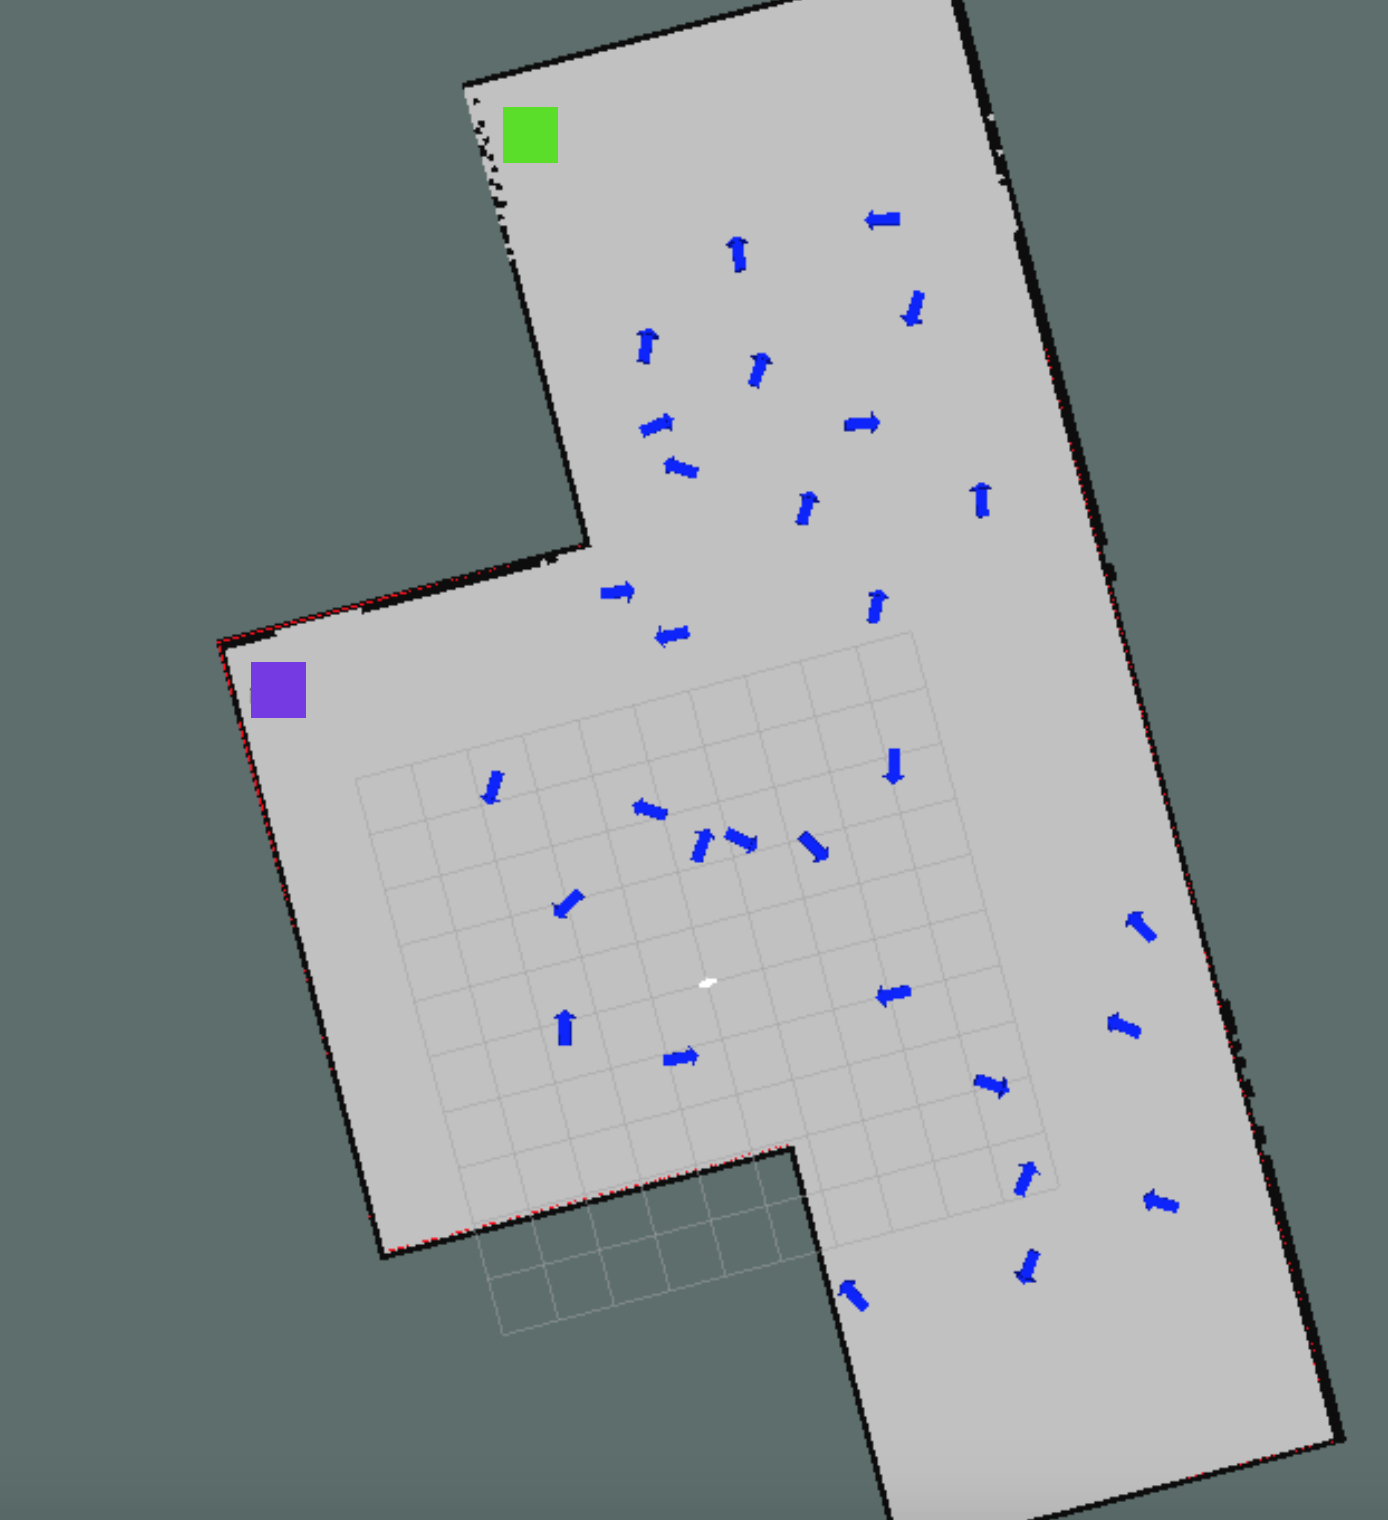
\includegraphics[scale = 0.15]{images/no_cf.png}
    \caption{Example setting }
    \label{fig:exp_setting}
  \end{subfigure}
  \hspace{10mm}
  \begin{subfigure}[b]{0.35\columnwidth}
  \hspace{4mm}
    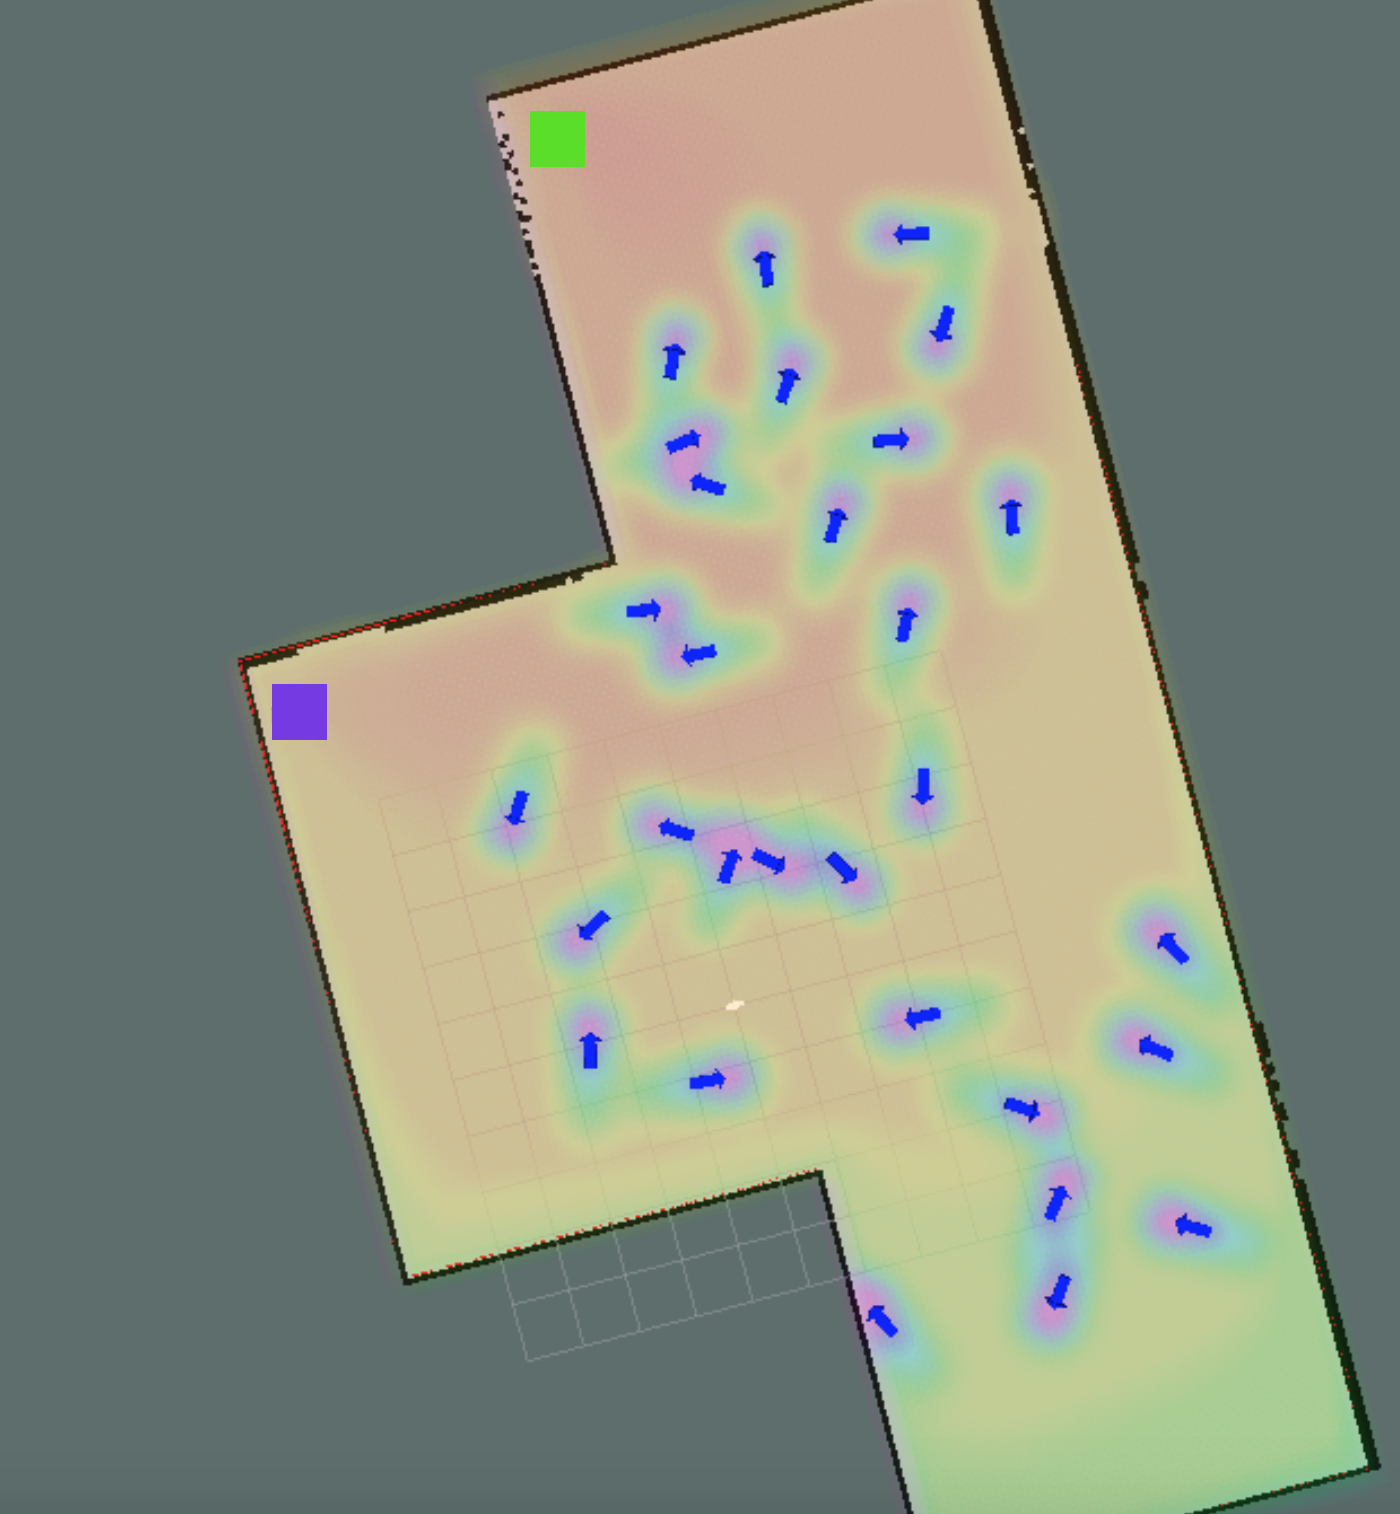
\includegraphics[scale = 0.15]{images/cf.png}
    \caption{Cost function}
    \label{fig:cost_f}
  \end{subfigure} 

  %\vspace{-3mm}
  \caption{(a) An instance of the randomised social navigation task. Arrows denote the position and orientation of people in the scene. The robot is represented by the box in magenta while the green box goal location. (b) The corresponding cost function. Red denotes \emph{low} cost, while purple denotes \emph{high} cost.}

    \vspace{-2mm}

  %\vspace{-3mm}
  \label{fig:setting}
  \end{figure}


% 	\begin{figure}[tbh]
% %	\hspace{-5cm}
% 	\centering
%       \begin{subfigure}[b]{0.42\columnwidth}
%     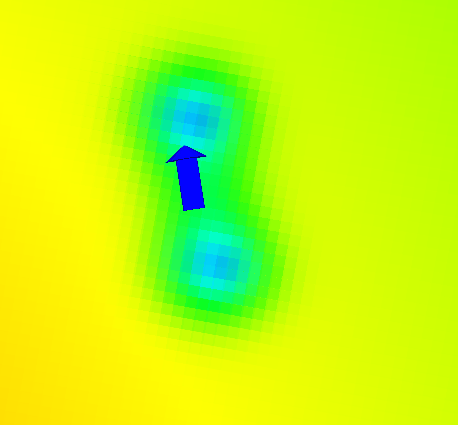
\includegraphics[scale=0.2]{images/person_feat2.png}
%     \caption{Social feature set S1.}
%     \label{fig:S1}
%   \end{subfigure}
%   \hspace{10mm}
%   \begin{subfigure}[b]{0.42\columnwidth}
%   \hspace{4mm}
%     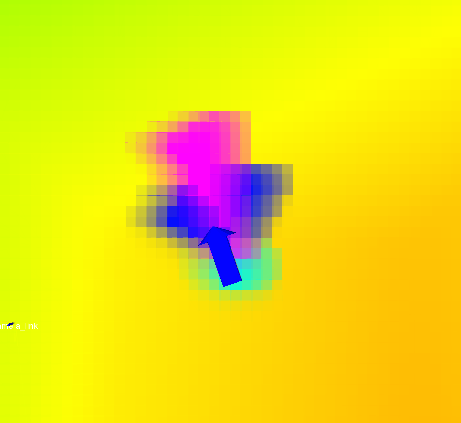
\includegraphics[scale=0.2]{images/person_feat1.png}
%     \caption{Social feature set S2}
%     \label{fig:S2}
%   \end{subfigure} 
%   %\vspace{-3mm}
%   \caption{Cost functions resulting from linear combinations of the social featuresets. Figure \ref{fig:S1} demonstrates featureset 1. It consists of three isotropic Gaussian functions centered in front in the center and behind the person. Figure \ref{fig:S2} shows the field-of-view features of featureset S2. \sw{I have no idea what these plots are showing.} \ks{Now?}}
%     \vspace{-2mm}
%   %\vspace{-3mm}
%   \label{fig:setting}
%   \end{figure}


	\subsubsection{Evaluation}

	To evaluate our algorithms, we generate a dataset $D$ by planning near-optimal paths from initial configurations $s_o$ to goal configurations $s_g$ under a ground-truth cost function $c_{gt}()$ derived from ground-truth weights $\mathbf{w}_{gt}$ and features $\mathbf{F}_{gt}$. A fully optimal path can only be derived asymptotically in terms of either time  for RRT$^*$, or resolution for A$^*$. In practice, however, we found that planning for 100 seconds using  RRT$^*$  achieves a path that is nearly optimal; running longer leads to negligible changes in path cost. 
	The resulting ground truth dataset enables a quantatitive empirical evaluation, which is otherwise problematic in IRL \cite{shiarlis2016inverse,vasquez2014inverse}. For each path $\zeta$ generated by the learning algorithm, we know its cost under the ground-truth cost function and features is simply  $\mathbf{w}_{gt}^T\mathbf{F}_{gt}(\zeta)$. Furthermore, we can compute the cost difference between the learned path and the demonstrated path with respect to ground truth:
	\begin{equation}
		Q(\zeta,\zeta_i,\mathbf{w}_{gt}) = \mathbf{w}_{gt}^T(\mathbf{F}_{gt}(\zeta)-\mathbf{F}_{gt}(\zeta_i)), \label{eq:obj_eval}
	\end{equation}
which is our primary performance metric.  Note that, if the demonstration path $\zeta_i$ is optimal under $\mathbf{w}_{gt}$, then $Q(\zeta,\zeta_i,\mathbf{w}_{gt}) \geq 0$. For our holonomic simulated experiments, we consider two learning scenarios.
\begin{enumerate}
	\item \textbf{Unknown weights}: only $\mathbf{w}_{gt}$ is unknown. The demonstrations and the learning algorithm share social feature set S1.
	\item \textbf{Unknown weights and features}: $\mathbf{w}_{gt}$ and $\mathbf{F}_{gt}$  are unknown. S2 is used to generate the demonstrations and S1 is used for learning.
\end{enumerate}

The first scenario evaluates each algorithm's ability to learn good cost functions when provided only with limited demonstrations of the task. The second scenario introduces a feature discrepancy to better simulate real-world settings, since it is unlikely that the features we define will exactly match those implicitly used by the human demonstrator.
% In both cases the ground-truth weights $\mathbf{w}_{gt}$ were chosen to induce a cost function that penalises passing in front of people. In addition, small weights were added to the person related features, as well as linear and exponential penalisation of the distance from the goal, so that the cost functions would not be too trivial. 

We also document the total learning time for K iterations for the algorithms under comparison.  All algorithms were implemented in Python, share similar functions, and were not optimised for speed apart from the caching scheme in RLT$^*$. Finally, we perform a qualitative evaluation by visually comparing the learned cost functions for each algorithm and the paths they generate against ground truth.

	\subsubsection{Holonomic Robot Results}

	Our dataset $D$ consists of 20 trajectories from random social social situations. We split $D$ into $D_{train}$ and $D_{test}$, each with 10 trajectories. After training on $D_{train}$, the cost difference of a cost function is evaluated on $D_{test}$ using \eqref{eq:obj_eval}. The process is repeated 7 times for the same dataset but with different random compositions of $D_{train}$ and $D_{test}$.  All learning algorithms are initialised using the same cost function that only favours shortest paths.
	
	As mentioned earlier, planning time and grid resolution affect the performance of RRT$^*$ and $A^*$, respectively. To make a fair comparison, we vary these two quantities for each algorithm and plot cost difference against learning time at each setting.  We can then identify which algorithms at which settings comprise the Pareto front, i.e., are undominated wrt cost difference and learning time.
	
	 Figures \ref{fig:res_sim1} and \ref{fig:res_sim2} show the results for the two scenarios described earlier. MMP\_X (green) refers to MMP with X meters of grid resolution while  RLT\_X (red) and RLT-NC\_X (blue) refer to RLT and RLT without caching, respectively, with X seconds of planning.  Since lower is better for both cost difference and learning time, the closer a point is to the bottom left corner, the better.
	 
	 RLT$^*$ (red) dominates a large portion of the Pareto front, demonstrating good performance and generalisation in reasonable time. Furthermore, caching not only speeds learning in RLT$^*$, it also modestly reduces cost differences. This suggests that the caching scheme introduces extra robustness and generalisation capabilities within the algorithm. As mentioned in Section \ref{subsec:cached} we believe that the caching scheme makes the gradients smoother and more consistent and thus serves as a type of momentum. To show this we plot the inner product between successive gradients during learning in Figure cite. We can see that the gradients of RLT$^*$ are clearly smoother, which further reinforces our claim. The performance of RLT$^*$ and RLT-NC significantly degrades at very low planning times (2 seconds) because AMMP cannot sample good enough paths to compute a useful gradient. Finally, MMP's learning time scales exponentially with the size of the grid. This, however, is not solely due to the graph getting larger but also because A$^*$ search scales poorly with the complexity of the cost function itself. Since it relies on an admissible heuristic that for complex cost functions is no longer tight, A$^*$ must expand many more states. By contrast, the sample-based RLT$^*$ is less susceptible to such problems.

	\begin{figure}[tbh]
	\centering
	\captionsetup[subfigure]{justification=centering}
	\hspace{-1cm}
      \begin{subfigure}[b]{0.41\columnwidth}
    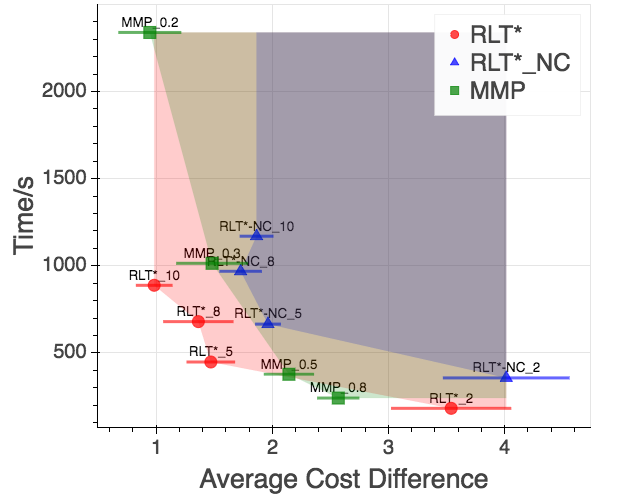
\includegraphics[scale=0.25]{images/pf_same.png}
    \caption{Unknown weights scenario.}
    \label{fig:res_sim1}
  \end{subfigure}
     	\hspace{10mm}
  \begin{subfigure}[b]{0.41\columnwidth}

    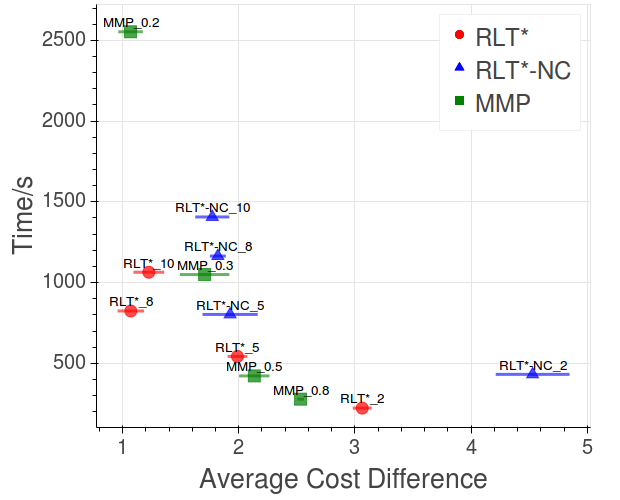
\includegraphics[scale=0.25]{images/pf_different.png}
    \caption{Unknown weights and features scenario.}
    \label{fig:res_sim2}
  \end{subfigure} 
    \caption{Learning time vs.\ cost difference on the holonomic robot for MMP (green), RLT-NC (blue), and RLT (red) at different planning fidelities. On both axes \emph{lower is better}.}
    \vspace{-2mm}
  %\vspace{-3mm}
  \label{fig:results_sim}
  \end{figure}



 	\begin{figure}[tbh]
%	\hspace{-5cm}
	\centering
    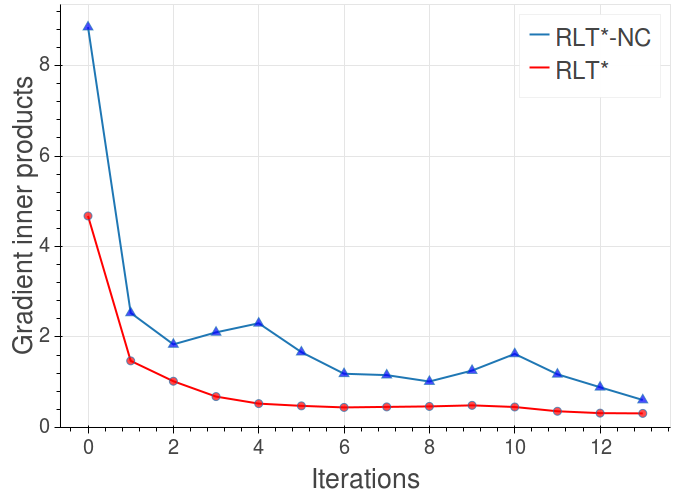
\includegraphics[scale=0.23]{images/momentum.png}
    \caption{Inner product of succcessive gradients during learning. The smoother curve for RLT$^*$ suggests that fixing the sampled points during learning introduces some notion of momentum. }
    \vspace{-2mm}
  %\vspace{-3mm}
  \label{fig:in_prod_grad}
  \end{figure}


	\begin{figure}[tbh]
%	\hspace{-5cm}
	\centering
    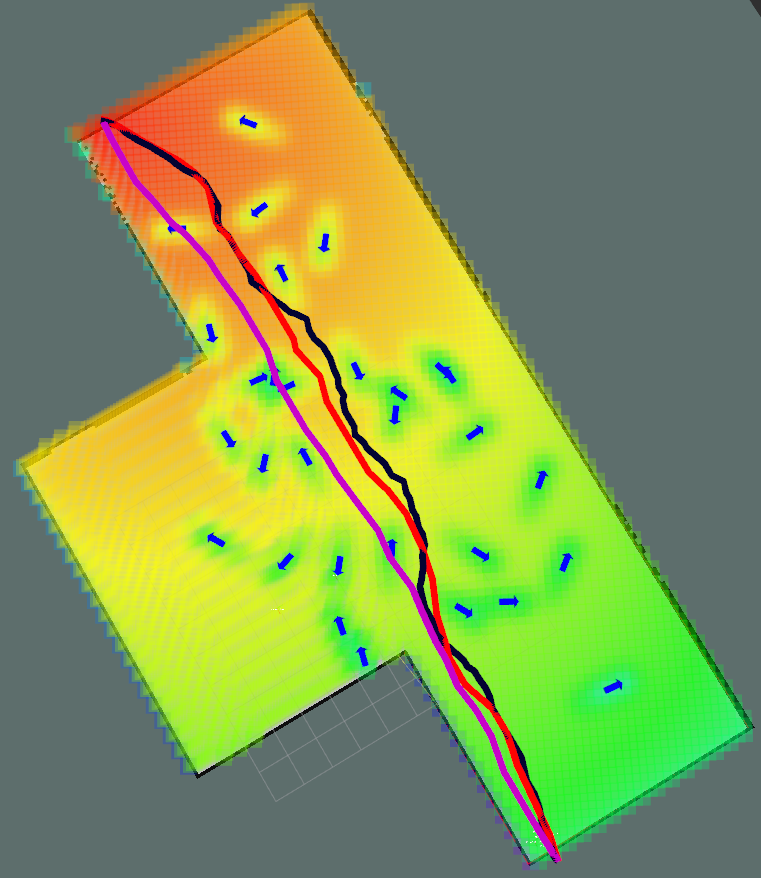
\includegraphics[scale=0.15]{images/cf_w_plans.png}
    \caption{Qualitative evaluation of simulated results. The colormap denotes the learned cost function. Red denotes \emph(low) cost and green \emph{high} cost. The learned path (red) is very similar to the demonstrated path (black) with a clear improvement over the path before learning (purple).}
    \vspace{-2mm}
  %\vspace{-3mm}
  \label{fig:results_qual}
  \end{figure}

  \subsubsection{Non-Holonomic Robot Results}
  As mentioned earlier, a potential advantage of RLT$^*$ is that it can efficiently handle learning in the case of motion constraints. In this paper we consider a robot planning in a three dimentional space, $(x,y,\theta)$, representing the position and orientation of the robot. The robot's motion is further subject to the following motion constraints:
%
  \begin{align}
  	&\dot{x} = v\times\cos(\theta),\\
  	&\dot{y} = v\times\sin(\theta),\\
  	&\dot{\theta} = \omega,
  \end{align}
  where $v,\omega$ are the linear and angular velocities respectively.
  To meet these constraints, we use the POSQ $\texttt{Steer}$ function \cite{palmieri2014novel}.  Since this approach gives a local closed-loop policy between two vertices of the tree, it is  more robust to noise and uncertainty in the motion. Furthermore, it has been shown to produce smooth paths between feasible configurations \cite{palmieri2014novel}. Evaluation is done in much the same way as in the previous section, except that we compare RLT$^*$ only to RLT-NC and not MMP, as the latter cannot handle motion constraints.
RLT-NC was given 100 seconds to plan, in which case about 3000 configurations were sampled, and RLT$^*$'s cache was set to this size. 

Figure \ref{fig:results_kino} shows that RLT$^*$ is an order of magnitude faster than RLT-NC, while achieving a lower cost difference. The kinematic constraints contribute to this speedup since they make the \texttt{Steer} and \texttt{Safe} procedures, which are cached, more expensive. As in the holonomic case, RLT$^*$ resulted in smoother learning supporting the results of Figure \ref{fig:in_prod_grad}. Figure \ref{fig:results_qual} shows an instance of the types of paths generated by our method when compared to ground truth. The specific example was drawn from the validation set and thus not a case of overfitting.
  	\begin{figure}[tbh]
	\centering
	\captionsetup[subfigure]{justification=centering}
	\hspace{-1cm}
      % \begin{subfigure}[b]{0.42\columnwidth}
    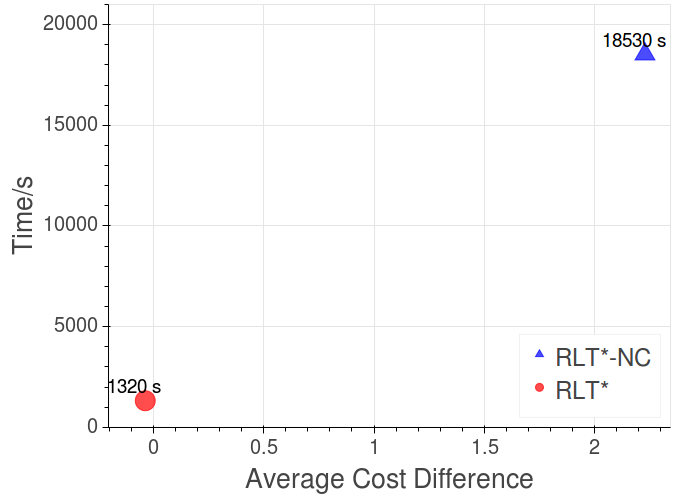
\includegraphics[scale=0.25]{images/pareto_front_kino.png}
    % \caption{Learning time vs.\ cost difference.}
    % \label{fig:res_kino1}
  % \end{subfigure}
     	% \hspace{10mm}
  % \begin{subfigure}[b]{0.42\columnwidth}

  %   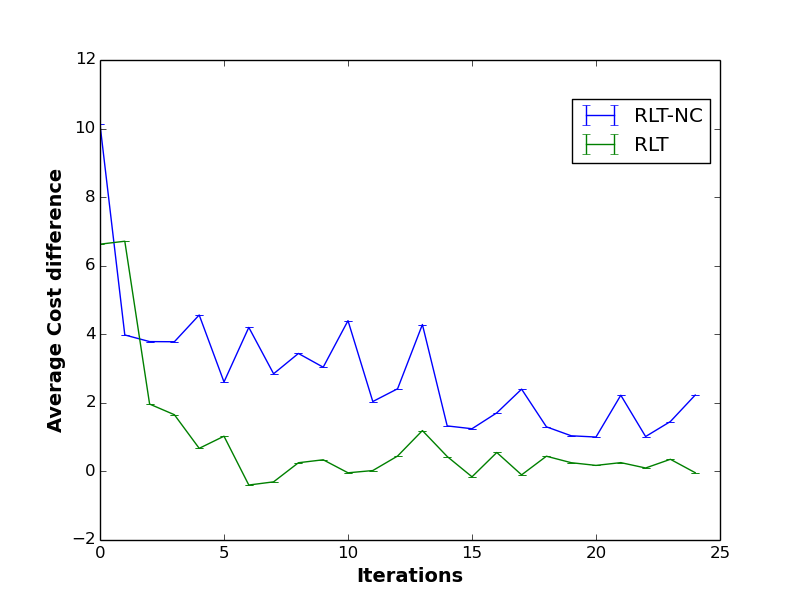
\includegraphics[scale=0.25]{images/cost_diff_val_kino.png}
  %   \caption{Learning curve}
  %   \label{fig:res_kino2}
  % \end{subfigure} 
    \caption{Non-holonomic robot results.}
    \vspace{-2mm}
  %\vspace{-3mm}
  \label{fig:results_kino}
  \end{figure}


	\subsection{Real Robot Experiments}
	In this section, we apply RLT$^*$ to real, human demonstrations using a telepresence robot in a social navigation scenario. Furthermore, we deploy the learned cost function on the actual robot.

	The experiments take place in a simplified version of the social scenarios we have seen in the previous section. There are two people in the scene at different positions and orientations. A human demonstrator is asked to execute paths for different initial and final conditions across the room. The task is similar to the one used in \cite{okallearning} and the purpose is to find cost functions that account for potential relationships between people depending on their orientation with respect to each other. For example, if people are facing each other, they are more likely engaged in conversation or some other activity (e.g., taking a photograph) and should not be interrupted. By contrast, if they are looking away from each other and there is enough distance between them then, it might be better to pass between them if doing so yields a shorter path.

	To collect data for learning and validation, we use an off-the-shelf telepresence system augmented with several sensors that allow localisation and perception \cite{shiarlis2015teresa}. We use an Optitrack motion-capture system to accurately collect ground truth data of both people robot positions. RLT$^*$ learns a cost function from this data using the social feature set S1 and the rest of the features described earlier.

Since quantitative evaluation is difficult using real data, as no ground truth is available, we perform a qualitative evaluation instead. Figure \ref{fig:results_real} shows some representative cases that arose during learning. Figure \ref{fig:res_real1} shows a case where RLT$^*$ produced paths (red) that are very similar to the demonstrated ones (black). Figure \ref{fig:res_real4} shows an instance instances where  the learned paths are reasonable even though they are not similar to the demonstrated paths.

			\begin{figure}[tbh]
%	\hspace{-5cm}
	\centering
      \begin{subfigure}[b]{0.42\columnwidth}
    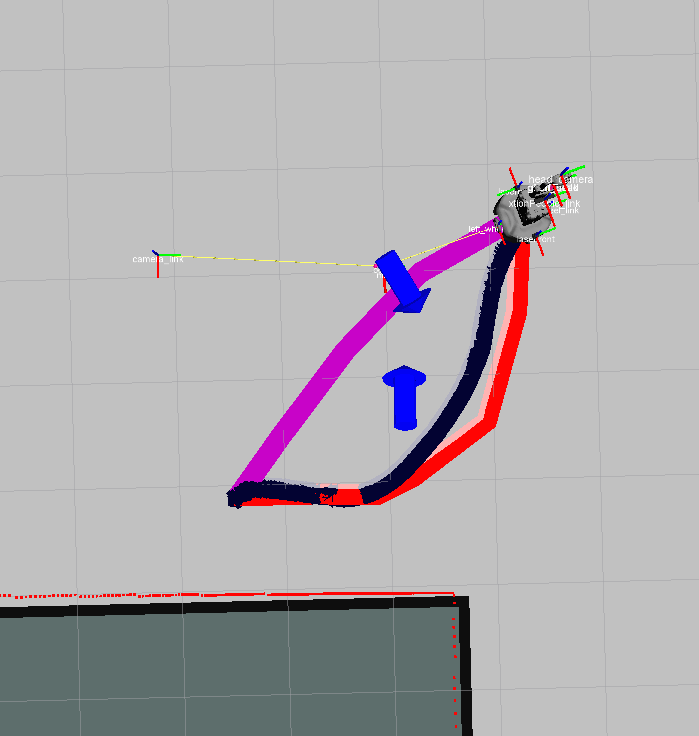
\includegraphics[scale=0.15]{images/real_good2.png}
    \caption{}
    \label{fig:res_real1}
  \end{subfigure}
  \hspace{10mm}
  \begin{subfigure}[b]{0.42\columnwidth}
  \hspace{4mm}
    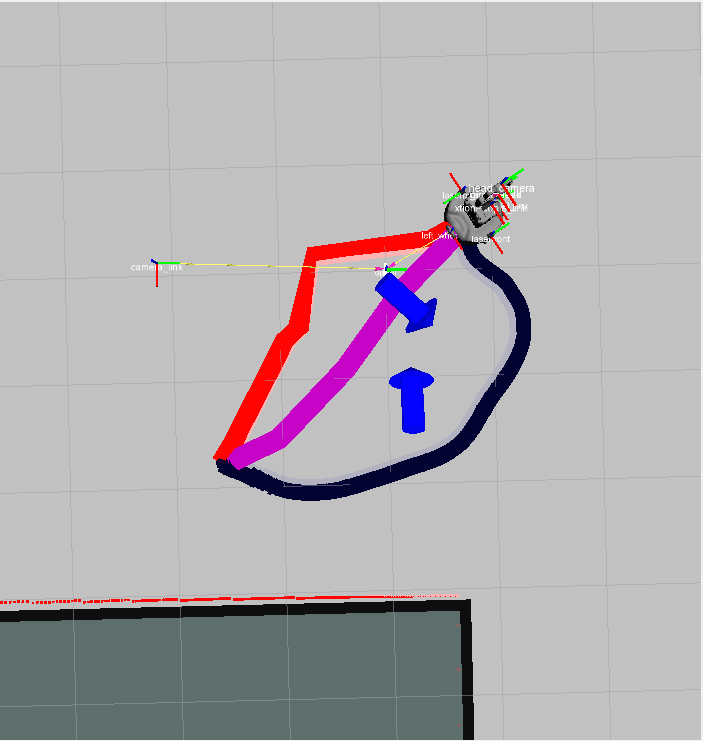
\includegraphics[scale=0.15]{images/real_reasonable3.png}
    \caption{}
    \label{fig:res_real4}
  \end{subfigure} 
    \caption{Real demonstrated paths (black), learned paths (red), and shortest paths (purple). In (a), the learned path is similar to the demonstrated path; in (b) it is different but reasonable.}
    \vspace{-2mm}
  %\vspace{-3mm}
  \label{fig:results_real}
  \end{figure}

	Finally, we succesfully deployed the learned cost function, shown in Figure \ref{fig:real_cf}, on a real telepresence robot. A video demonstrating this deployment can be found in the supplementary material. Even though our planner outputs a full policy in terms of angular and linear velocities, to follow the prescribed path we used an elastic bands local planner in order to deal with dynamic changes in the environment.\ks{should I say this?} 

	\begin{figure}[tbh]
%	\hspace{-5cm}
	\centering
    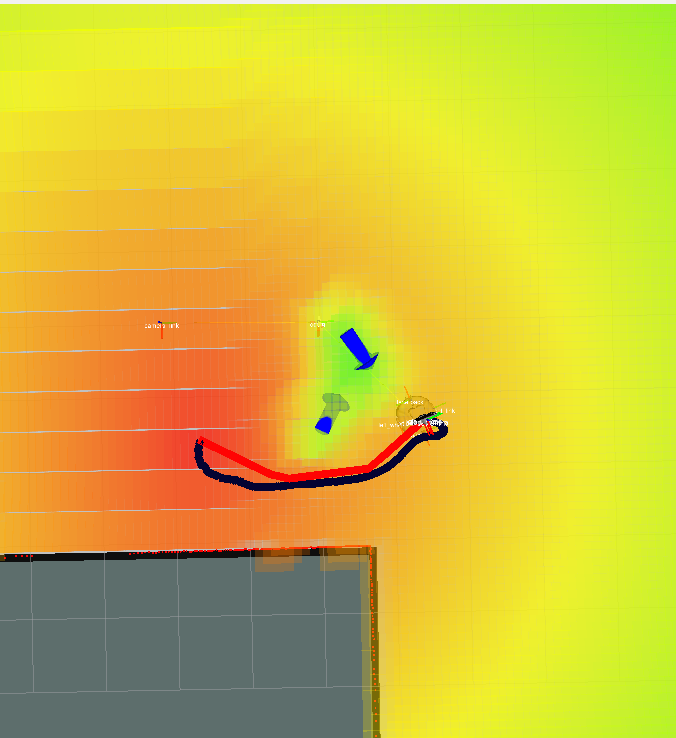
\includegraphics[scale=0.15]{images/cf_real.png}
    \caption{Cost function learned using data from real demonstrations on a telepresence robot.}
    \vspace{-2mm}
  %\vspace{-3mm}
  \label{fig:real_cf}
  \end{figure}





	% For a qualitative comparison, we look to Figures \ref{fig:path_compare} and \ref{fig:cfs}. Figure \ref{fig:path_compare} shows a demonstrated path (black) along with the paths generated by three of the four algorithms. Note the effect of planning on a coarse grid in the case of MMP$_{0.8}$ (green). We can also see that RLT$^*$ (red) more faithfully replicates the example path. Figure \ref{fig:cfs} compares the ground truth cost function (Figure \ref{fig:get_cf}) against the learned cost functions for  MMP$_{0.3}$ and RLT$^*$ (Figures \ref{fig:astar03_cf}, \ref{fig:rrt_cf}). This comparison shows that  MMP$_{0.3}$ overestimates the cost related with the distance from the goal, i.e., the cost increases faster as we move away from the goal. This yields paths that reach the goal earlier, possibly accounting for the small difference in performance between the two algorithms. 

% \begin{figure}[tbh]
% 	\vspace{-4mm}
% 	\centering
% %	\hspace{-5cm}
%       	\hspace{-12mm}
%       \begin{subfigure}[b]{0.43\columnwidth}

%     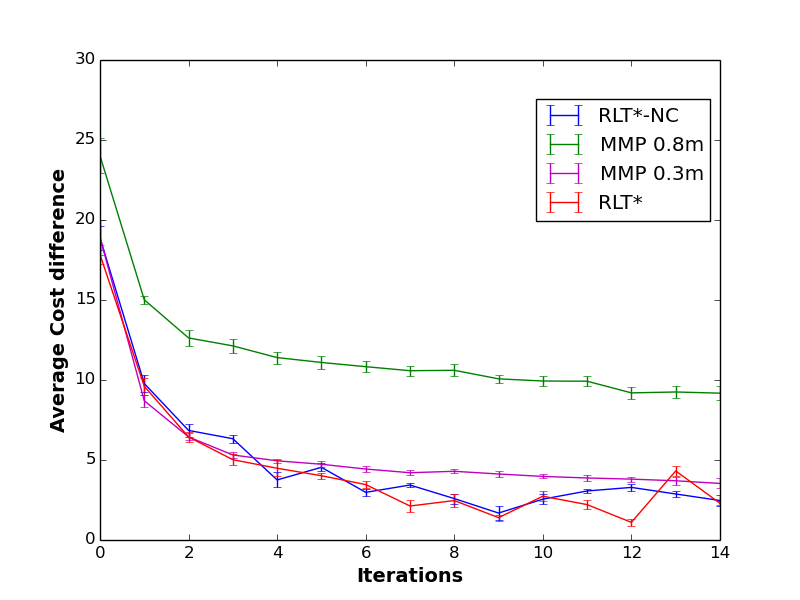
\includegraphics[clip=true,width=1.30\textwidth]{images/cost_diff_train.png}
%     \caption{Train}
%     \label{fig:train_results}
%   \end{subfigure}
%  % \hspace{5mm}
%  \hspace{5mm}
%   \begin{subfigure}[b]{0.43\columnwidth}
%     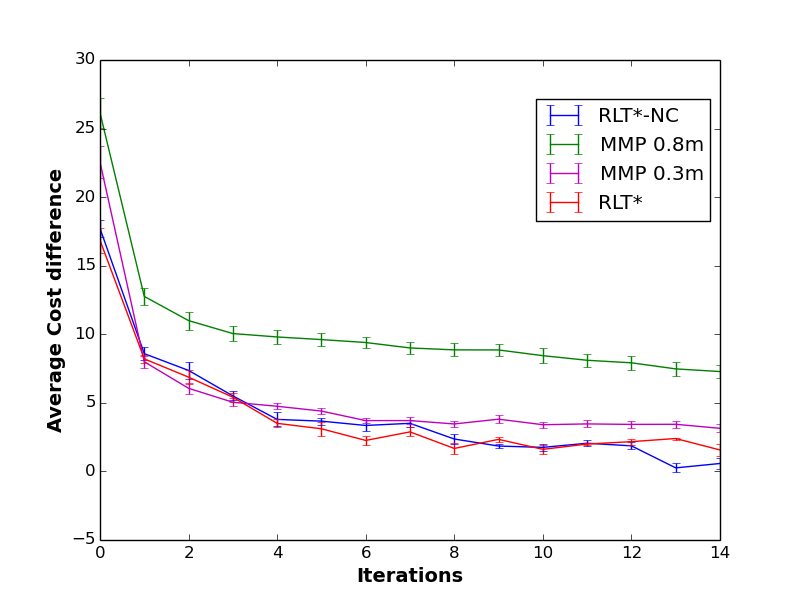
\includegraphics[clip=true,width=1.30\textwidth]{images/cost_diff_val.png}
%     \caption{Test}
%     \label{fig:test_results}

%   \end{subfigure} 

%   %\vspace{-3mm}
%   \caption{Train and test set average cost difference, for 15 iterations. Error bars represent standard error over four independent runs on shuffled versions of the data. (RLT$^*$-NC is RLT$^*$ without caching.)}
%   \vspace{-1mm}
%   \label{fig:results}
% \end{figure}



% 	\begin{table}[]
% 	\scalebox{0.82}{
% 	\begin{tabular}{|l|l|l|l|l|}
% 	\hline
% 	               & MMP$_{0.8}$     & MMP$_{0.3}$       & RLT$^*$-NC  & RLT$^*$ \\ \hline
% 	Iteration (s) & 1.83(0.79) & 20.93(12.14) & 12(0) & 5.87(0.50)  \\ \hline
% 	Learning (s) & 275.2      & 3140.6       & 1808  & 911.7       \\ \hline
% 	$Q(\zeta,\zeta_i,\mathbf{w}_{gt})$ & 7.28      & 3.14       & 0.57  & 1.57       \\ \hline
% 	\end{tabular}}
% 	\caption{Per iteration and total learning times for our proposed algorithms and the baselines (RLT$^*$-NC is RLT$^*$ without caching.)}
% 	\label{tab:time}
% 	\end{table}


	% \begin{figure}
	% \centering
	% %\vspace{-3.3mm}
	%     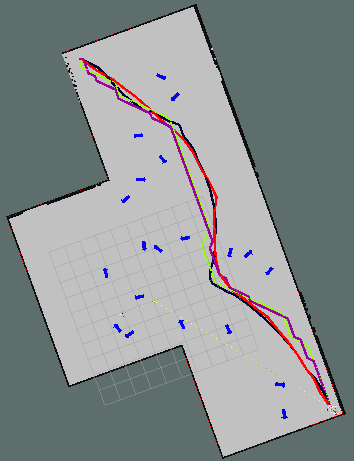
\includegraphics[width=0.22\textwidth,height = 39mm ]{images/path_compare.png}
	% %\vspace{-4mm}
	%   \caption{Qualitative comparison of paths. Goal is at the top left, robot begins on the bottom right. Black: demonstration path. Red: RLT$^*$. Green: MMP$_{0.8}$, Magenta: MMP$_{0.3}$ }
	%   \label{fig:path_compare}
	%   \vspace{-2mm}
	% \end{figure}


	% \begin{figure}[tbh]
	% \hspace{5mm}
 %      \begin{subfigure}[b]{0.309\columnwidth}
 %    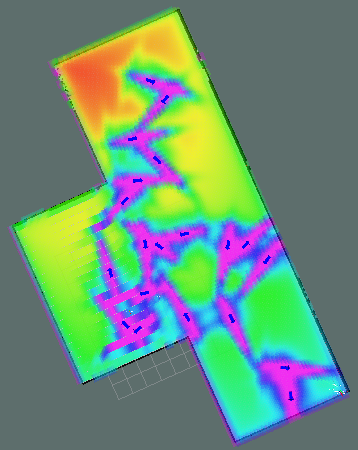
\includegraphics[width=1.\textwidth,height = 32mm]{images/gt_ct.png}
 %    \caption{Ground truth}
 %    \label{fig:get_cf}
 %  \end{subfigure}
 %  %\hspace{1mm}
 %  \begin{subfigure}[b]{0.30\columnwidth}
 %    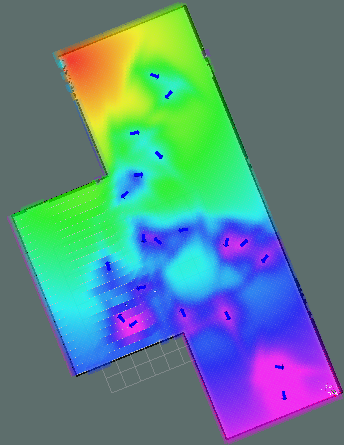
\includegraphics[width=1.\textwidth,height = 32mm]{images/astar03.png}
 %    \caption{MMP$_{0.3}$}
 %    \label{fig:astar03_cf}
 %   \end{subfigure}
 %   %\hspace{1mm}
 %  \begin{subfigure}[b]{0.305\columnwidth}
 %    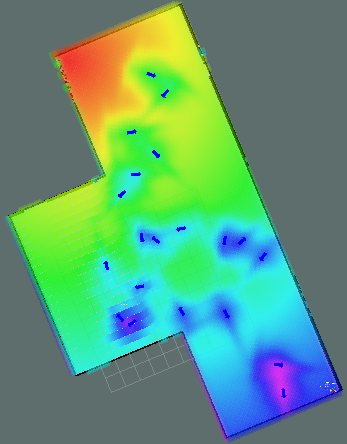
\includegraphics[width=1.\textwidth,height = 32mm]{images/rrt_cf.png}
 %    \caption{RLT$^*$}
 %    \label{fig:rrt_cf}
 %  \end{subfigure} 
 %  	  \caption{Ground truth and learned cost functions using MMP$_{0.3}$ and RLT$^*$.  \label{fig:cfs}}
 %  \end{figure}

\vspace{-1mm}
\section{Conclusion \& Future Work}
In this paper, we proposed the Rapidly Exploring Learning Trees (RLT$^*$), which learns the cost functions of Rapidly Exploring Random Trees (RRT) from demonstration, thereby making inverse learning methods applicable to more complex tasks. Our approach extends the Maximum Margin Planning to work with RRT$^*$ cost functions. Furthermore, it uses a caching scheme that greatly reduces the computational cost and improves performance. Our results in simulated social navigation scenarios show that RLT$^*$ achieves better performance at lower computational cost, even when there is a discrepancy between the features used for demonstration and learning. Furthermore, our results show that RLT$^*$ can handle more complex configuration spaces with motion constraints. Finally, we used RLT$^*$ to learn a cost function using data from real demonstrations on a telepresence robot and successfully deployed that cost function back on the robot.

In future work, we hope to extend RLT$^*$ to model how features evolve over time, in order to, e.g., consider people's movement during planning.  For complex social path planning applications, periodic replanning has been shown to help \cite{vasquez2014inverse,henry2010learning}. Replanning in RRT$^*$ is also possible \cite{otte2015rrtx} and could potentially be incorporated into RLT$*$.

\bibliographystyle{IEEEtran}
\bibliography{references}



\end{document}
